\documentclass{beamer}

\mode<presentation>
{
  \usetheme{Berkeley}
  \setbeamercovered{transparent}
}

\usepackage[absolute,overlay]{textpos}
\usepackage{graphicx}
\usepackage{color}
\usepackage{epsfig}
\usepackage[english]{babel}
\usepackage{listings}
\usepackage{graphics}
\usepackage{subfigure}

\setlength{\TPHorizModule}{1cm}
\setlength{\TPVertModule}{\TPHorizModule}
\textblockorigin{1cm}{1cm} % start everything near the top-left corner
\setlength{\parindent}{0pt}

\title{Data Dissemination: from Academia to Industry}

\author{\textbf{Jo{\~a}o Leit{\~a}o}\\NOVA-LINCS \& NOVA University of Lisbon 
\\\textbf{Jordan West}\\BASHO Inc.
}
\date{RICON\\Las Vegas\\October 2014}

\begin{document}
%\definecolor{links}{rgb}{0.2116,0.0104,0.7716}
%\definecolor{highlight}{rgb}{1,1,0.1}


\frame{

\titlepage

}

\section{Motivation}

\frame
{
	\frametitle{Outline}
{
\small
	\tableofcontents[hideallsubsections]
}
}

\frame
{
	\frametitle{Outline}
{
\small
	\tableofcontents[currentsection,hideallsubsections]
}
}

\frame{

\frametitle{Motivation}
\framesubtitle{Data Dissemination}

\begin{block}{Classical Distributed Systems Challenge}
How to disseminate information across a large number of participants?
\end{block}

\pause

\begin{itemize}
\item Some intuitive requirements:
\begin{itemize}
	\item Reliable.
	\item Efficient.
	\item Scalable.
\end{itemize}
\end{itemize}

}

\frame{

\frametitle{Motivation}
\framesubtitle{Data Dissemination}

\begin{block}{Applications}
\begin{itemize}
	\item Notification systems.
	\item Streaming multimedia content.
	\item \emph{Cluster Management}
\end{itemize}
\end{block}

\pause

\begin{block}{In practice...}
When I started to think about this problem, I was mostly focused on peer-to-peer systems.
\end{block}}

\section{The Academic View: Data Dissemination}

\frame
{
	\frametitle{Outline}
{
\small
	\tableofcontents[currentsection,hideallsubsections]
}
}

\frame
{
	\frametitle{Outline}
{
\small
	\tableofcontents[currentsection,hideallsubsections]
}
}

\subsection{Design Alternatives: One to All}

\frame{
\frametitle{The Academic View: Data Dissemination}
\framesubtitle{Design Alternatives: One to All}

\begin{figure}[h]
  \begin{center}
  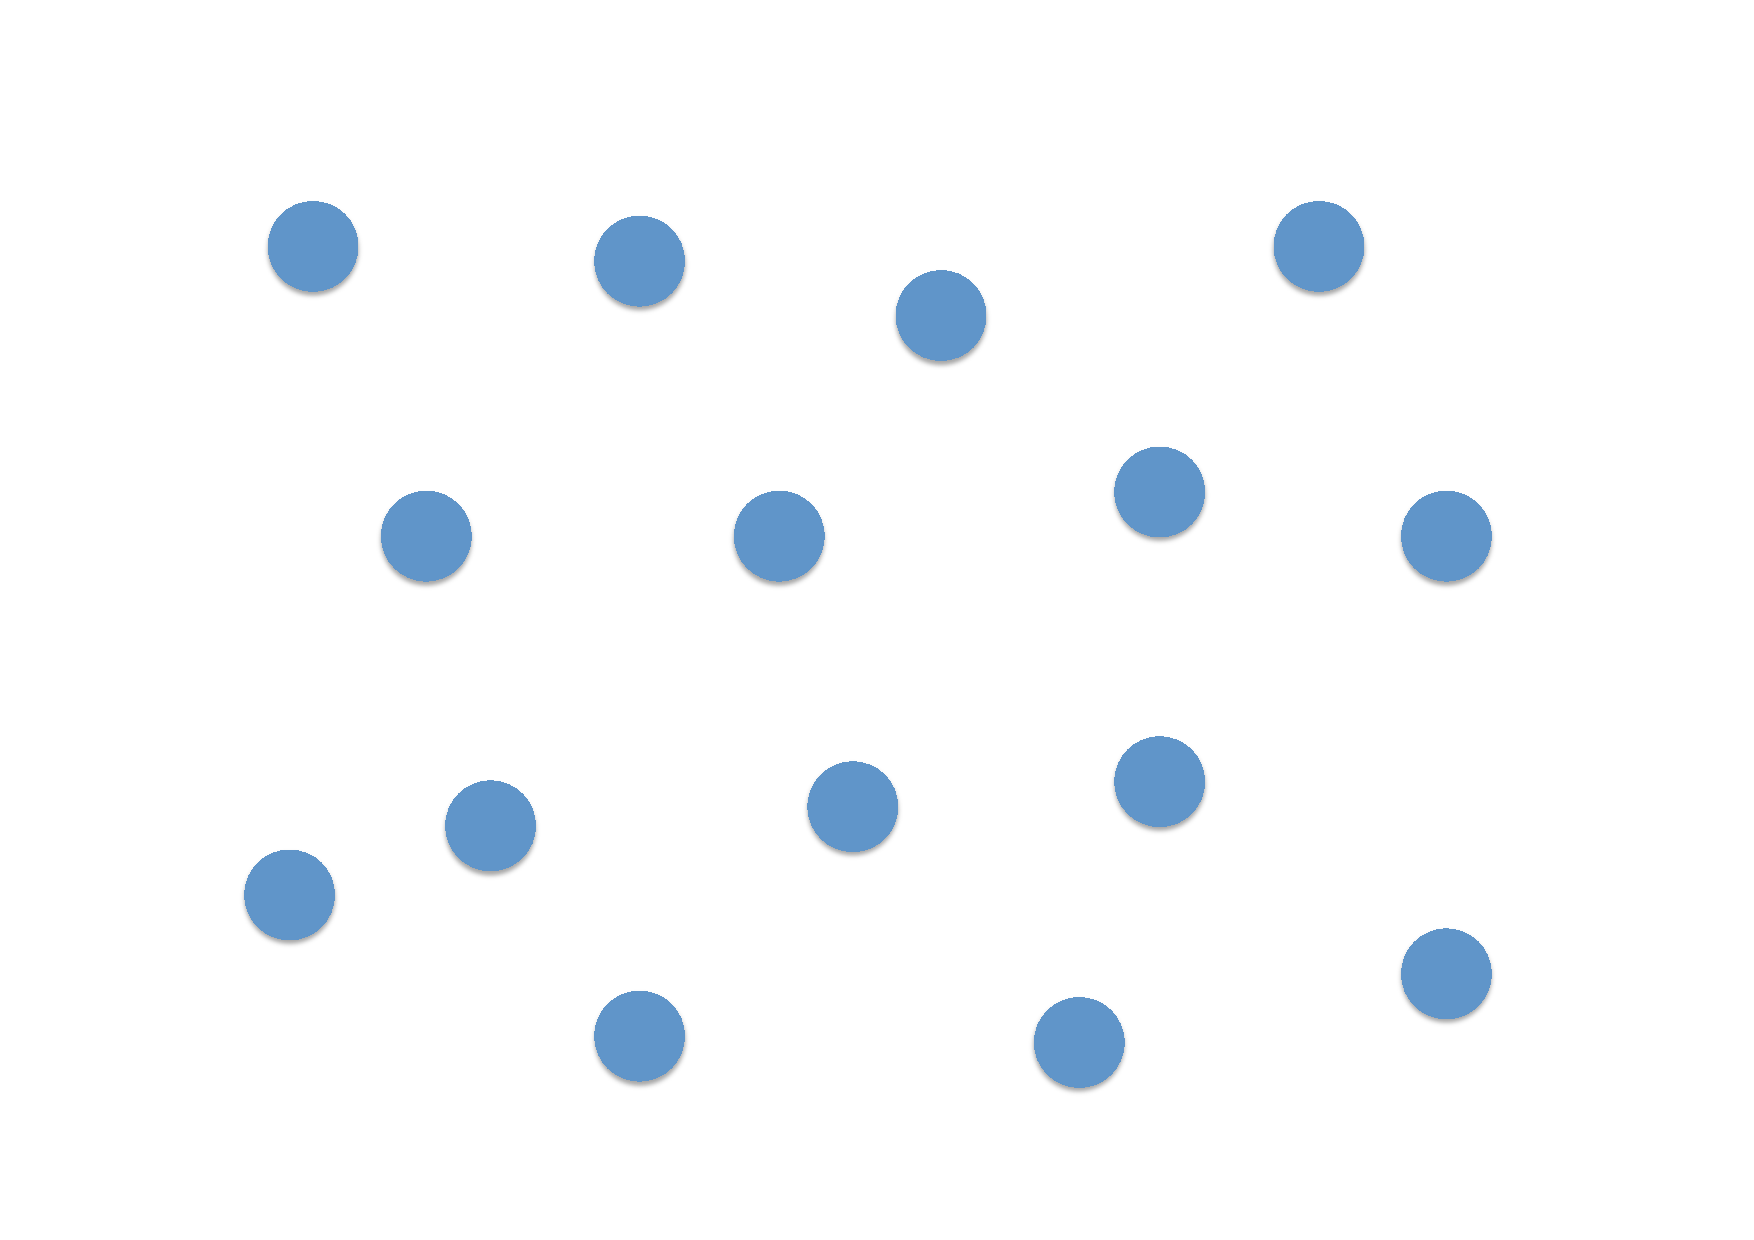
\includegraphics[width=1\textwidth]{pics/one2all1}
  \end{center}
\end{figure}

}

\frame{
\frametitle{The Academic View: Data Dissemination}
\framesubtitle{Design Alternatives: One to All}

\begin{figure}[h]
  \begin{center}
  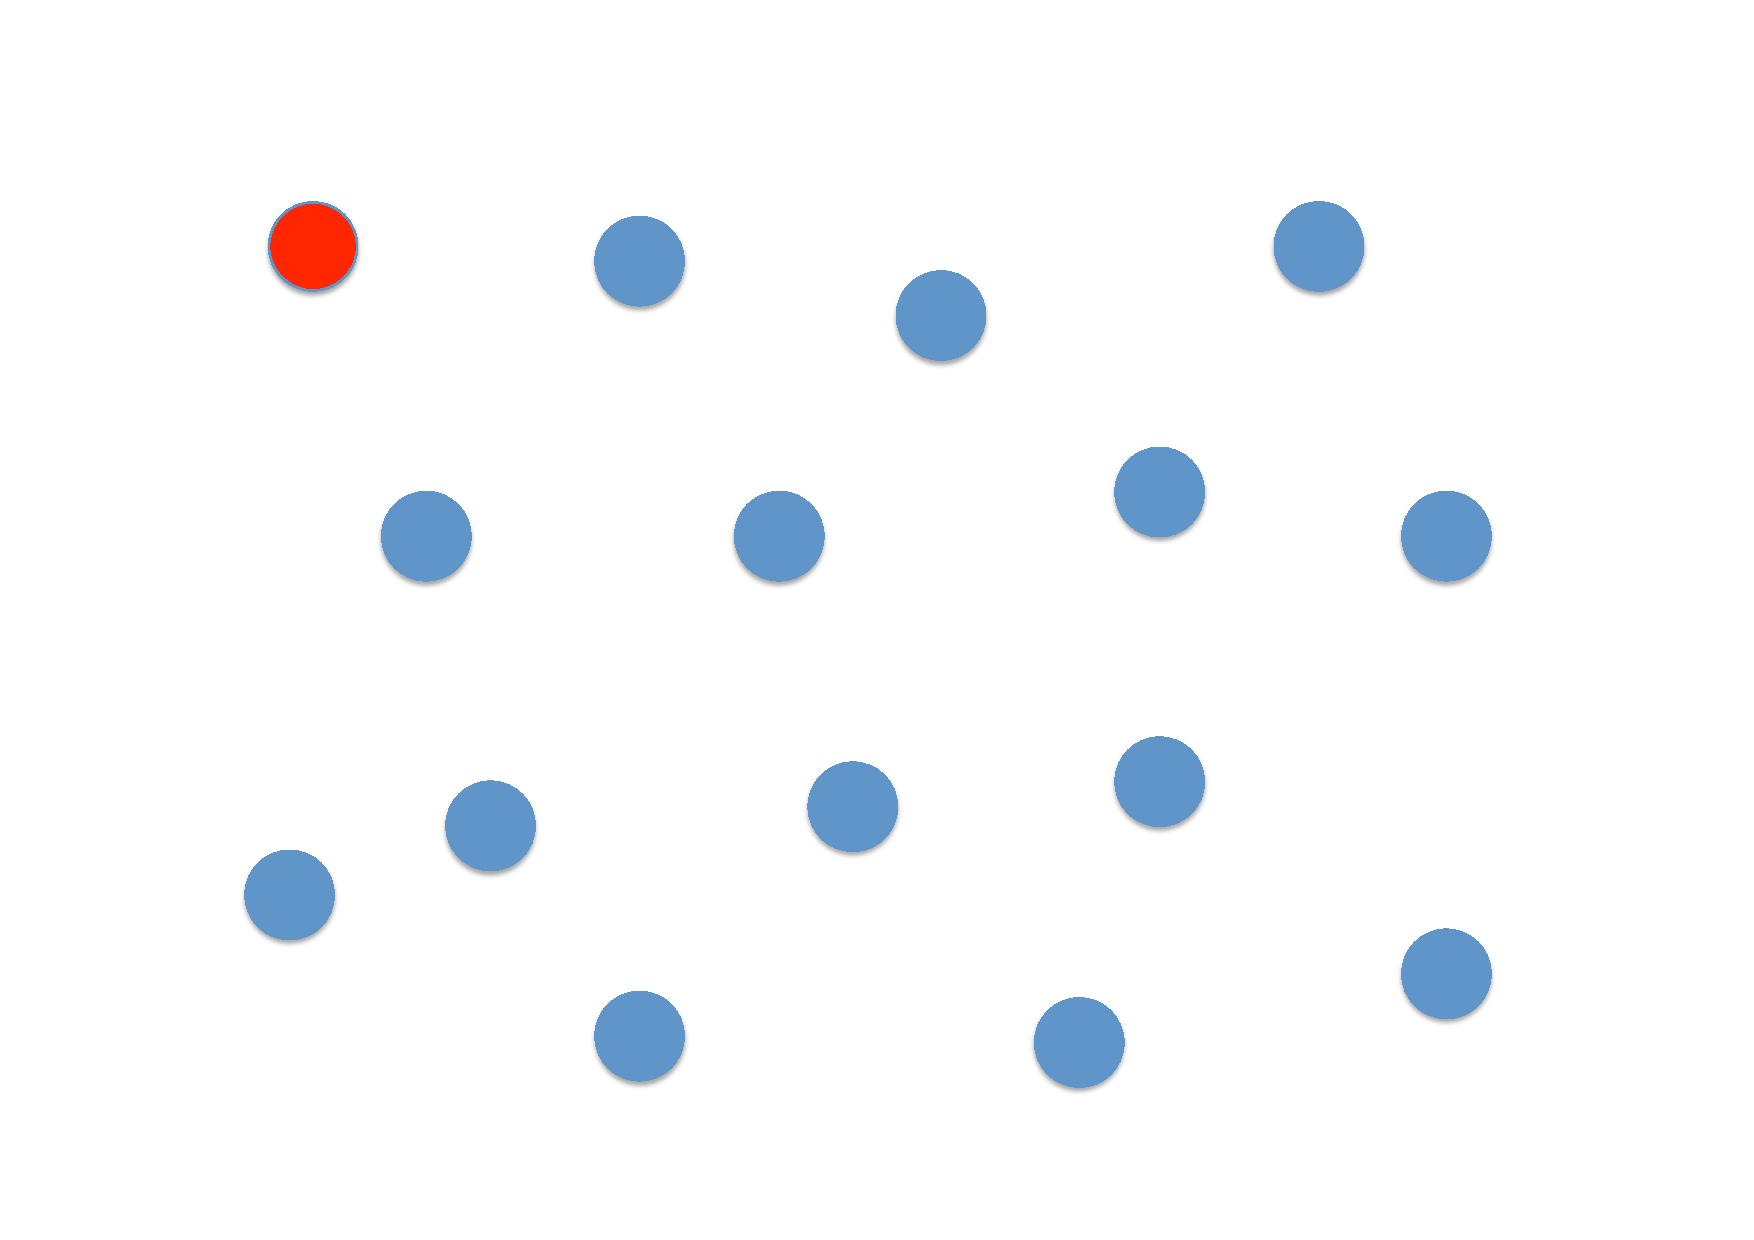
\includegraphics[width=1\textwidth]{pics/one2all2}
  \end{center}
\end{figure}

}

\frame{
\frametitle{The Academic View: Data Dissemination}
\framesubtitle{Design Alternatives: One to All}

\begin{figure}[h]
  \begin{center}
  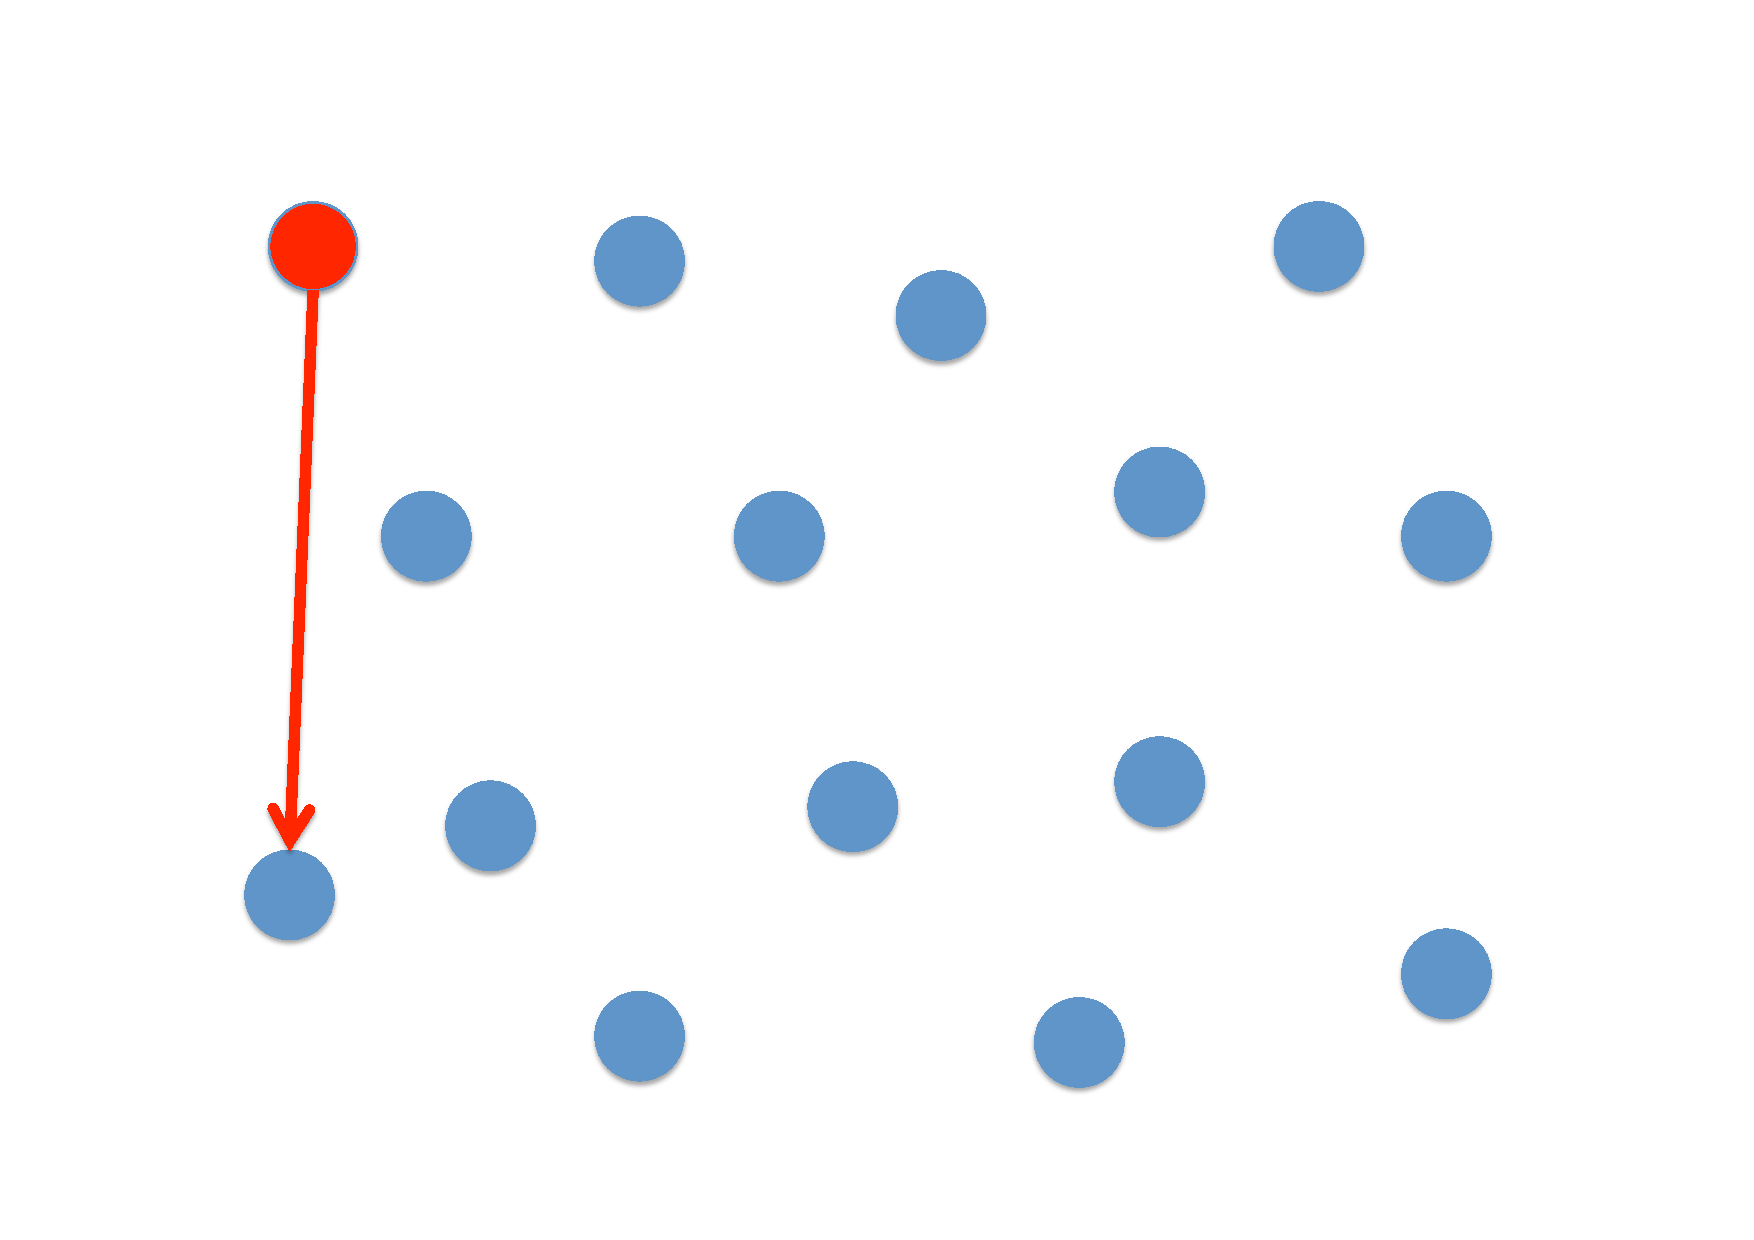
\includegraphics[width=1\textwidth]{pics/one2all3}
  \end{center}
\end{figure}

}

\frame{
\frametitle{The Academic View: Data Dissemination}
\framesubtitle{Design Alternatives: One to All}

\begin{figure}[h]
  \begin{center}
  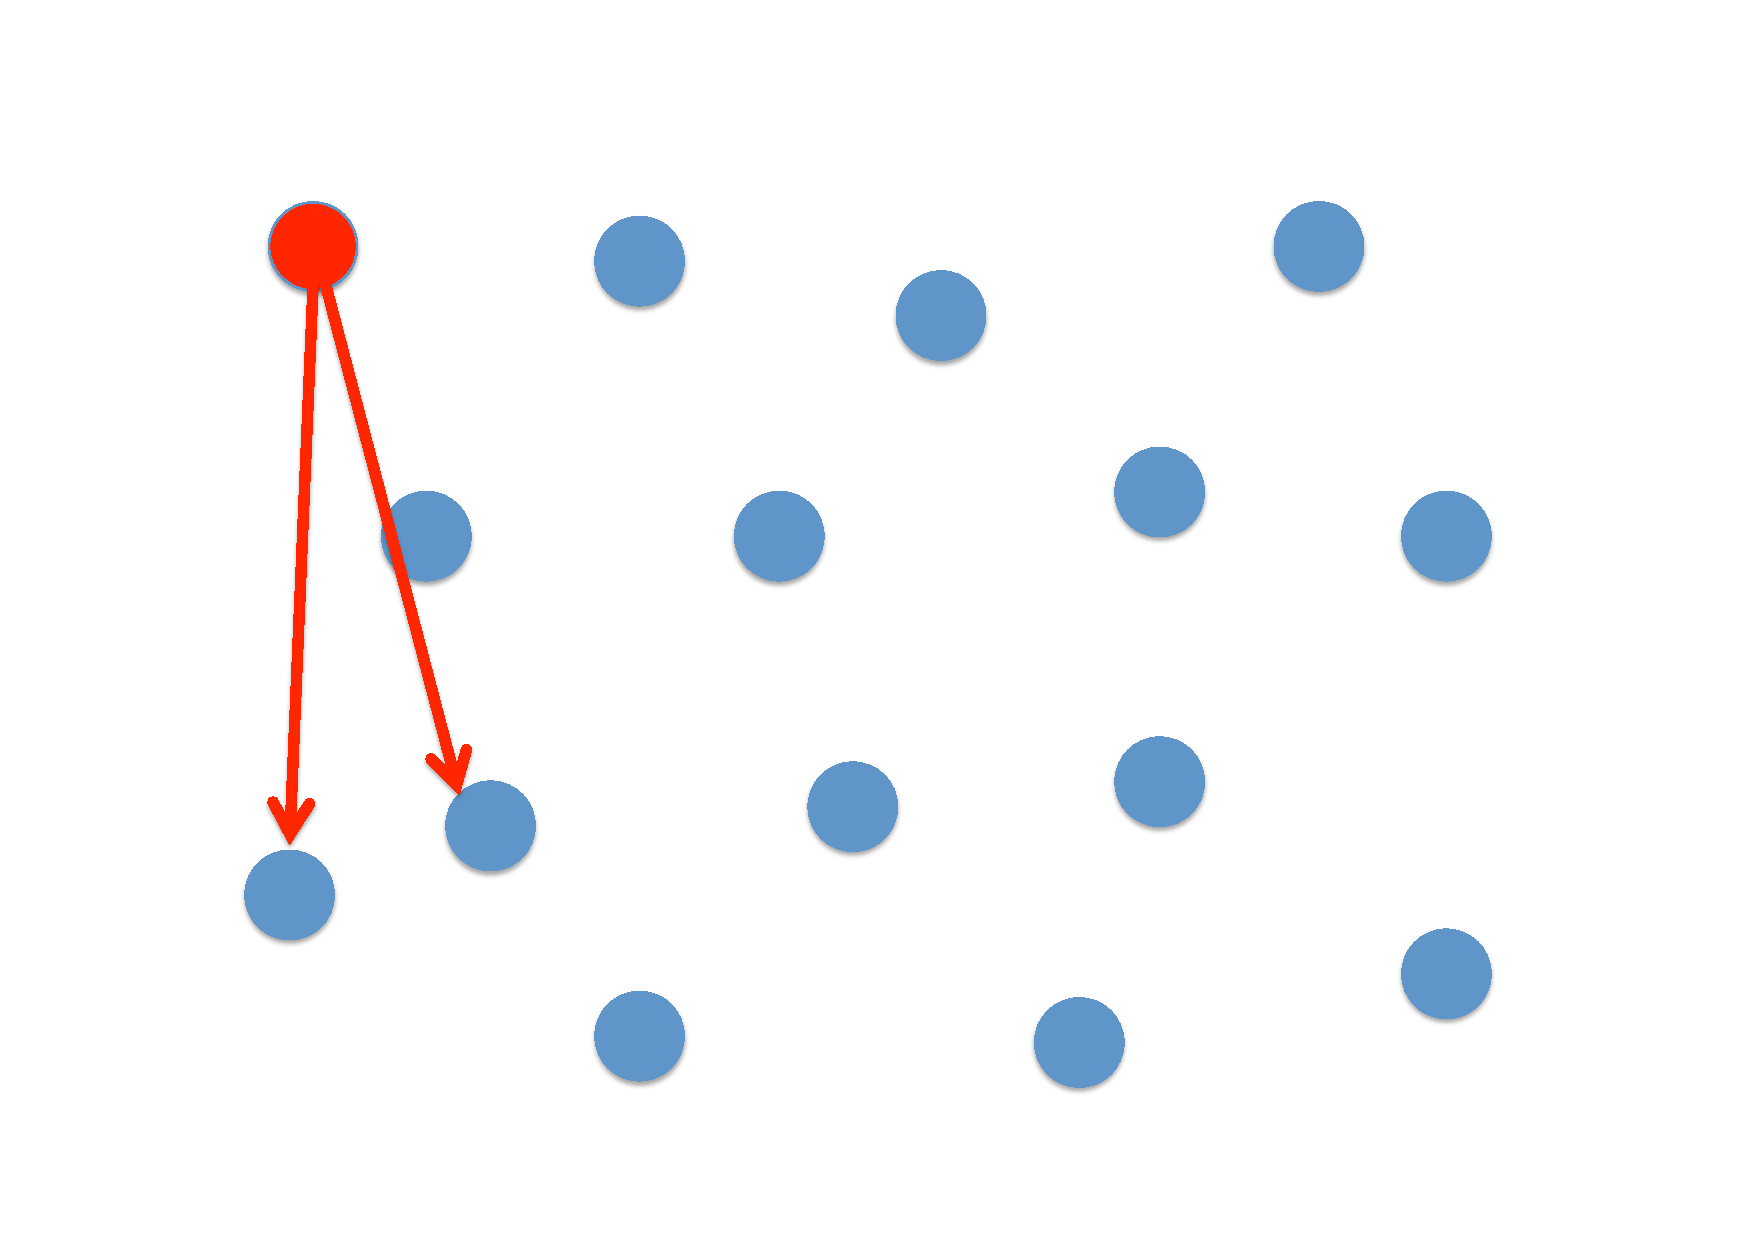
\includegraphics[width=1\textwidth]{pics/one2all4}
  \end{center}
\end{figure}

}

\frame{
\frametitle{The Academic View: Data Dissemination}
\framesubtitle{Design Alternatives: One to All}

\begin{figure}[h]
  \begin{center}
  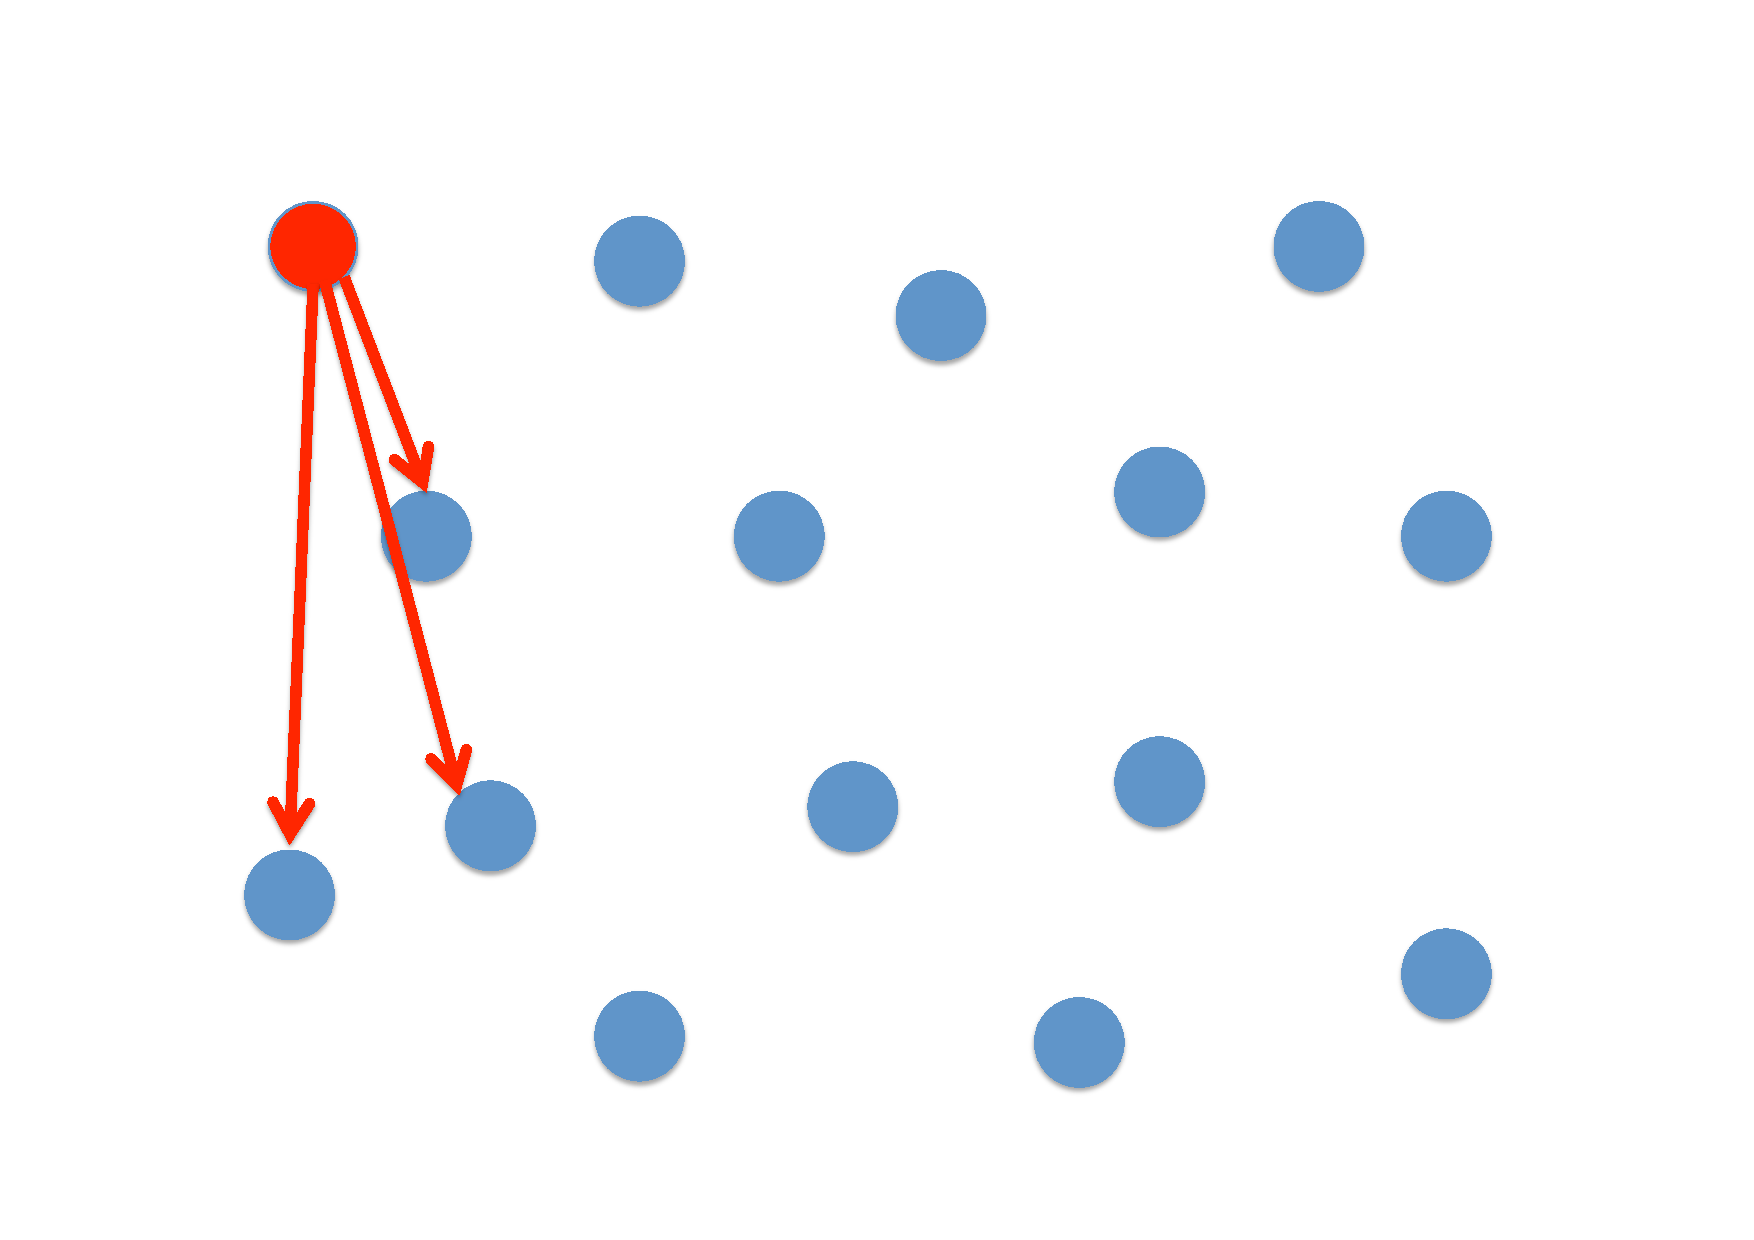
\includegraphics[width=1\textwidth]{pics/one2all5}
  \end{center}
\end{figure}

}

\frame{
\frametitle{The Academic View: Data Dissemination}
\framesubtitle{Design Alternatives: One to All}

\begin{figure}[h]
  \begin{center}
  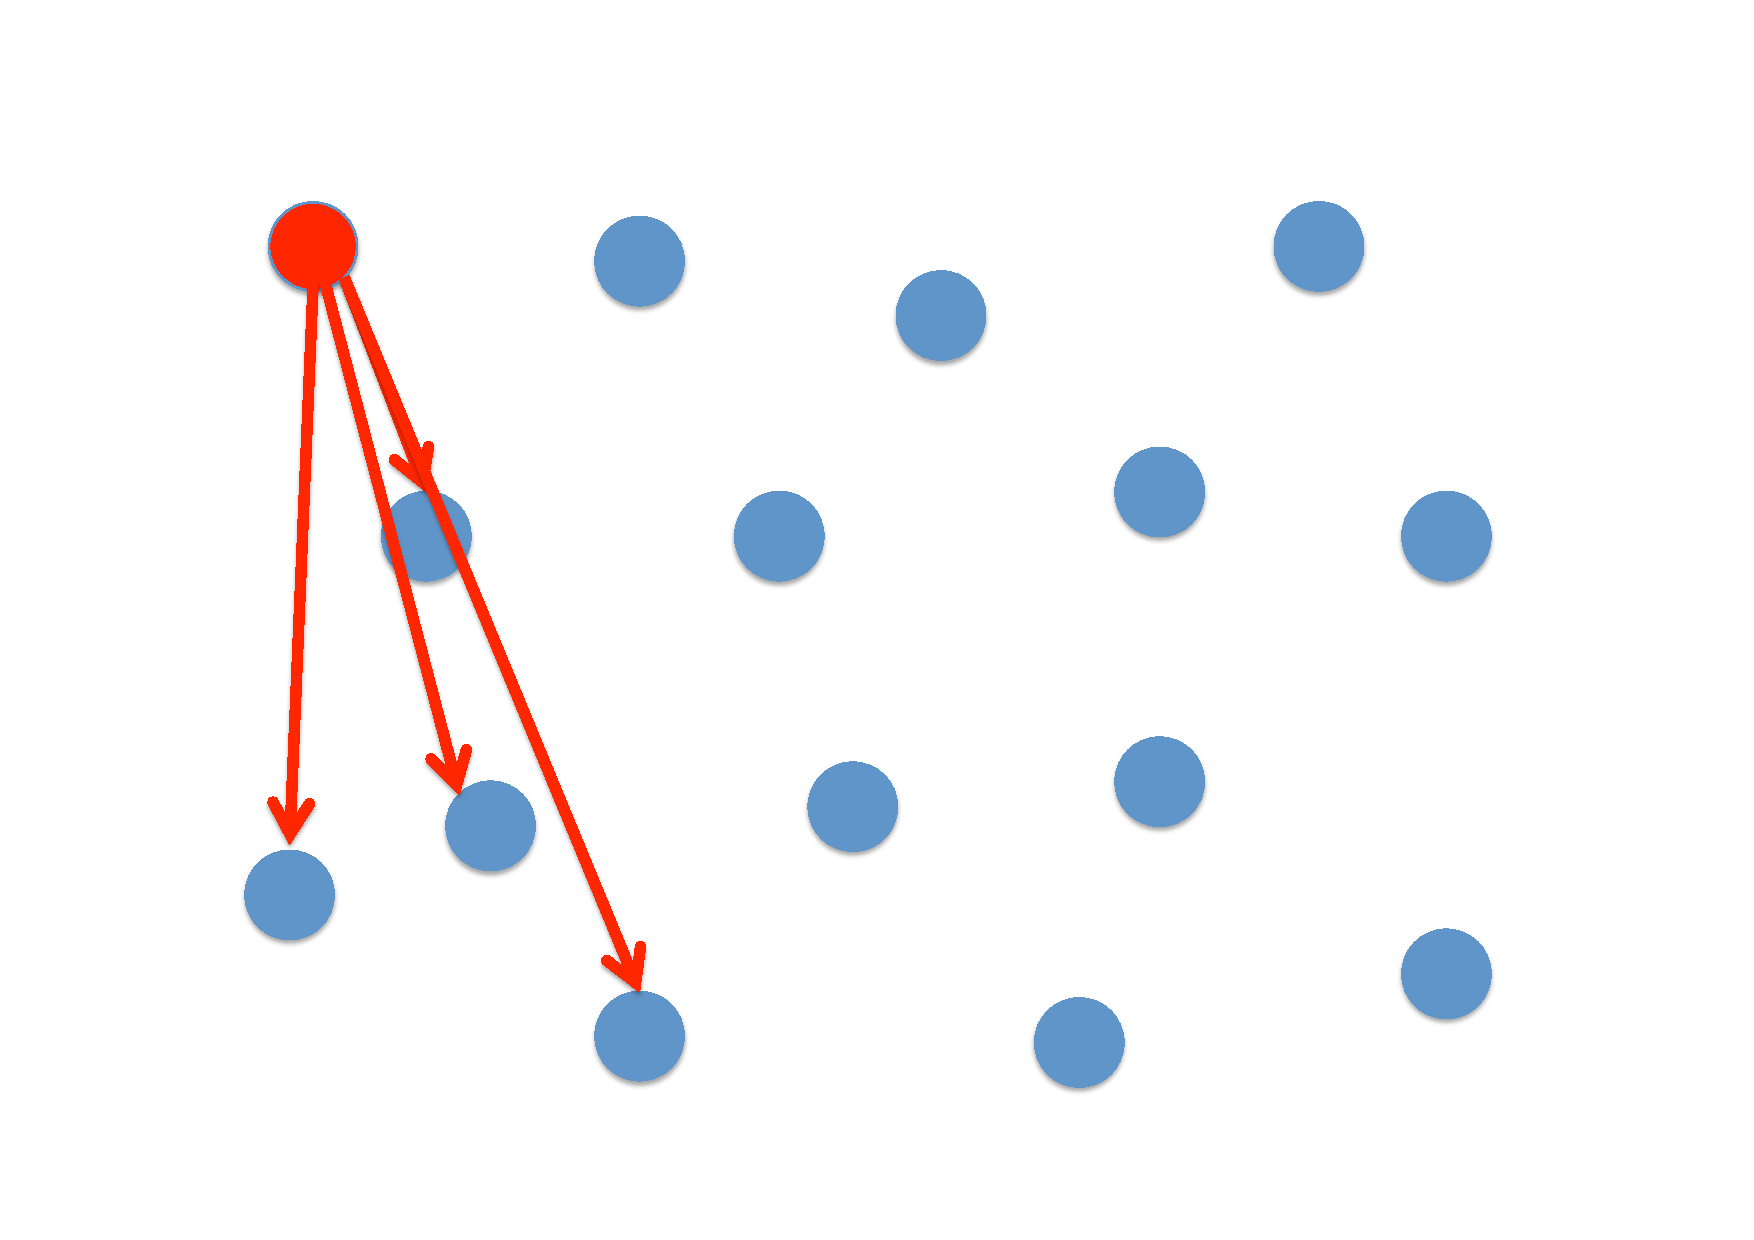
\includegraphics[width=1\textwidth]{pics/one2all6}
  \end{center}
\end{figure}

}

\frame{
\frametitle{The Academic View: Data Dissemination}
\framesubtitle{Design Alternatives: One to All}

\begin{figure}[h]
  \begin{center}
  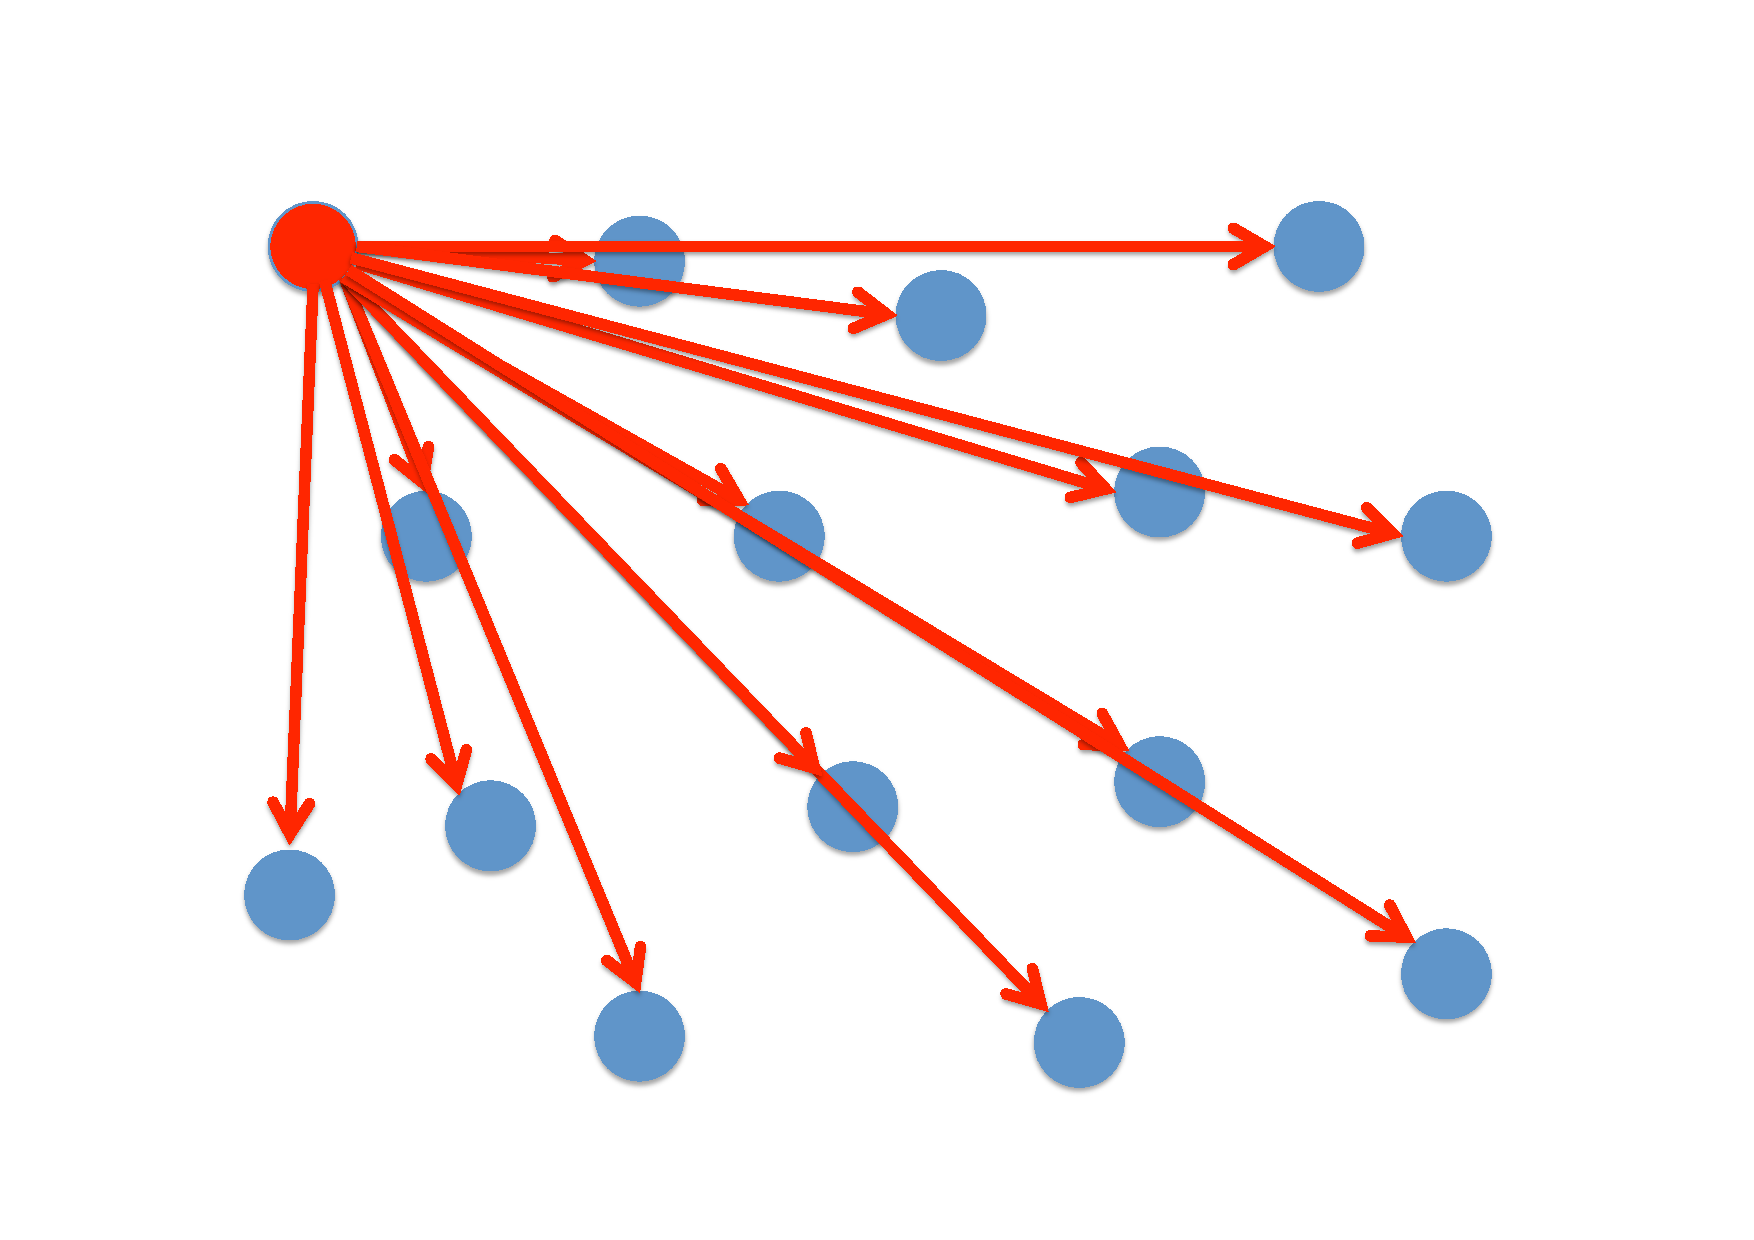
\includegraphics[width=1\textwidth]{pics/one2all7}
  \end{center}
\end{figure}

}

\frame{
\frametitle{The Academic View: Data Dissemination}
\framesubtitle{Design Alternatives: One to All}

\begin{block}{One to All}
	\begin{itemize}
		\item Positive
		\begin{itemize}
			\item Straight forward.
			\item No redundancy (i.e, each node receives each message a single time).
		\end{itemize}
	\end{itemize}
	
	\pause
	
	\begin{itemize}
		\item Negative Aspects:
		\begin{itemize}
			\item Requires each node to know the full membership.
			\item Not Scalable (no load distribution).
			\pause
			\item Not Resilient to Faults.
		\end{itemize}
	\end{itemize}
}

\frame{
\frametitle{The Academic View: Data Dissemination}
\framesubtitle{Design Alternatives: One to All}

\begin{figure}[h]
  \begin{center}
  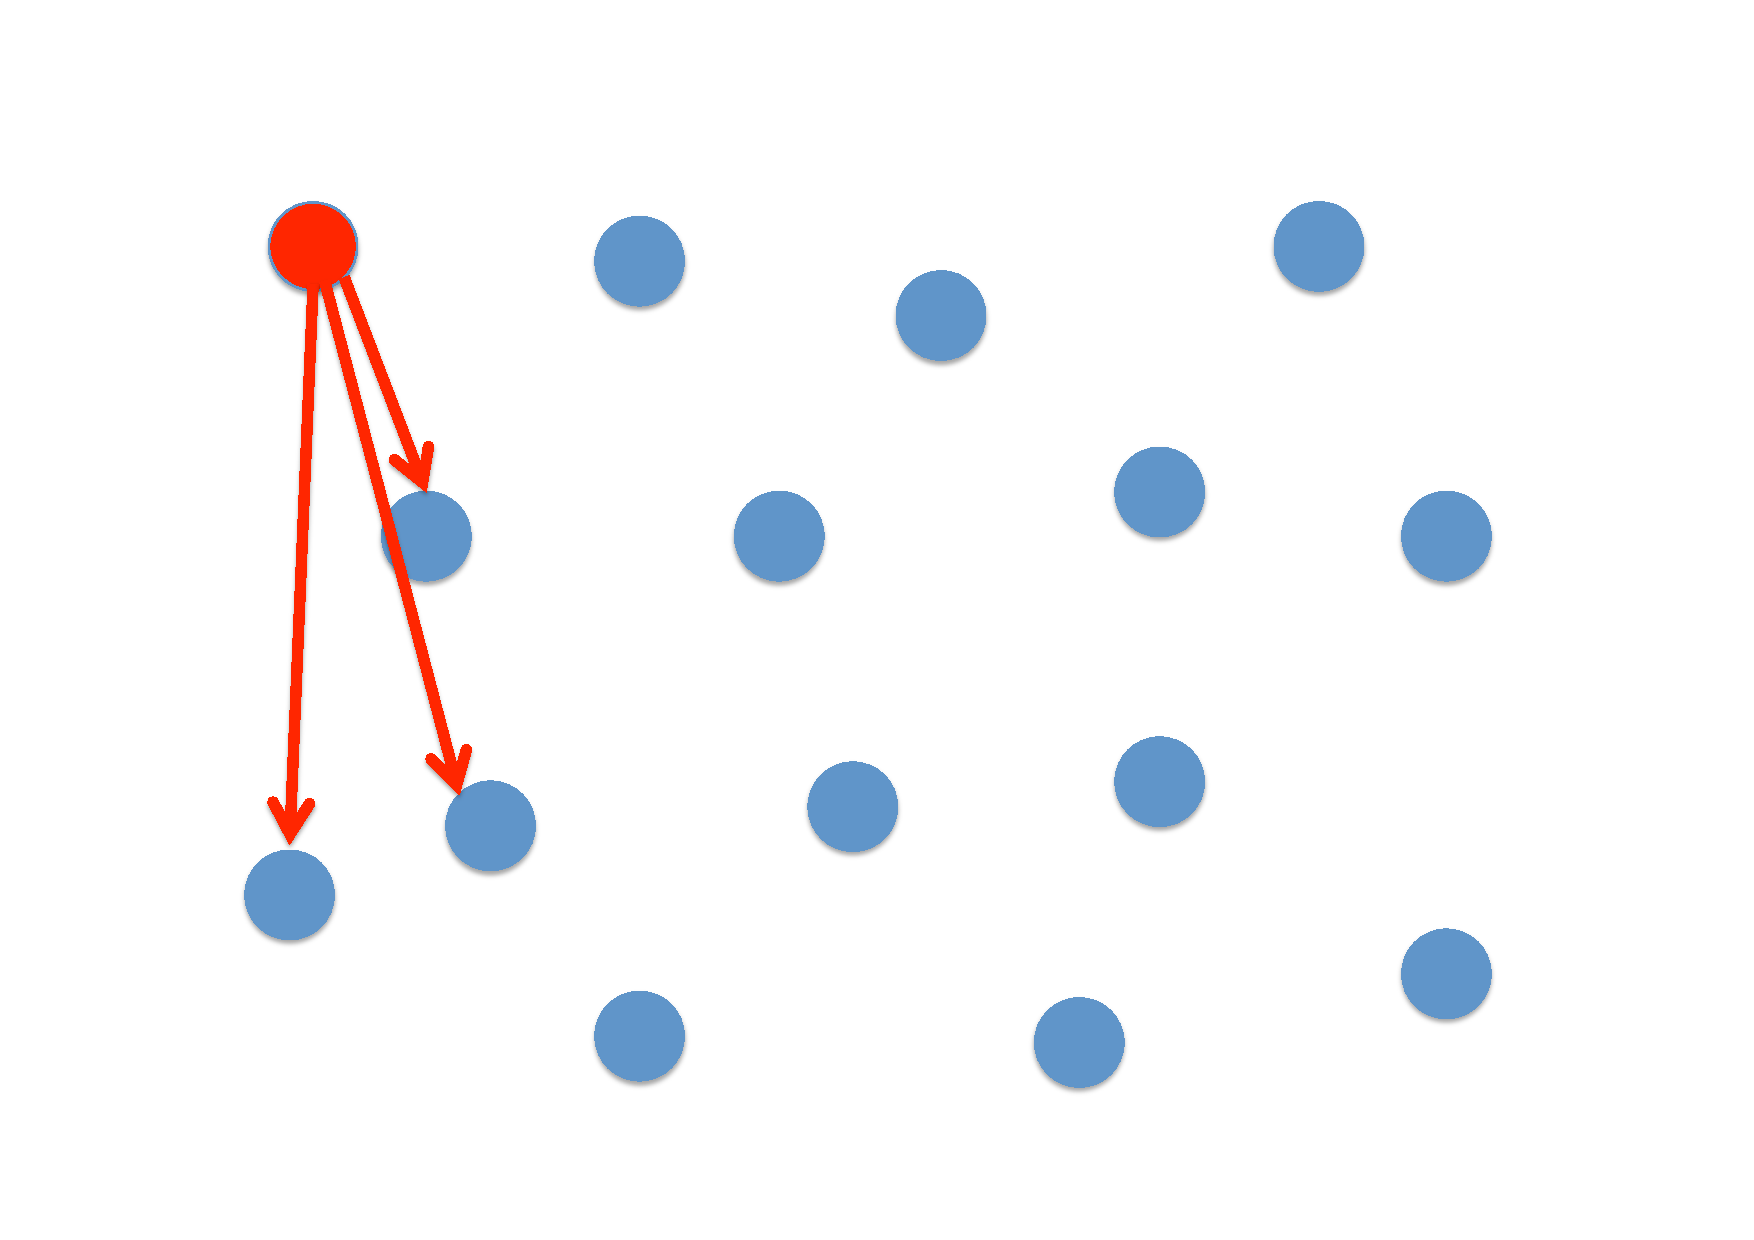
\includegraphics[width=1\textwidth]{pics/fault1}
  \end{center}
\end{figure}

}

\frame{
\frametitle{The Academic View: Data Dissemination}
\framesubtitle{Design Alternatives: One to All}

\begin{figure}[h]
  \begin{center}
  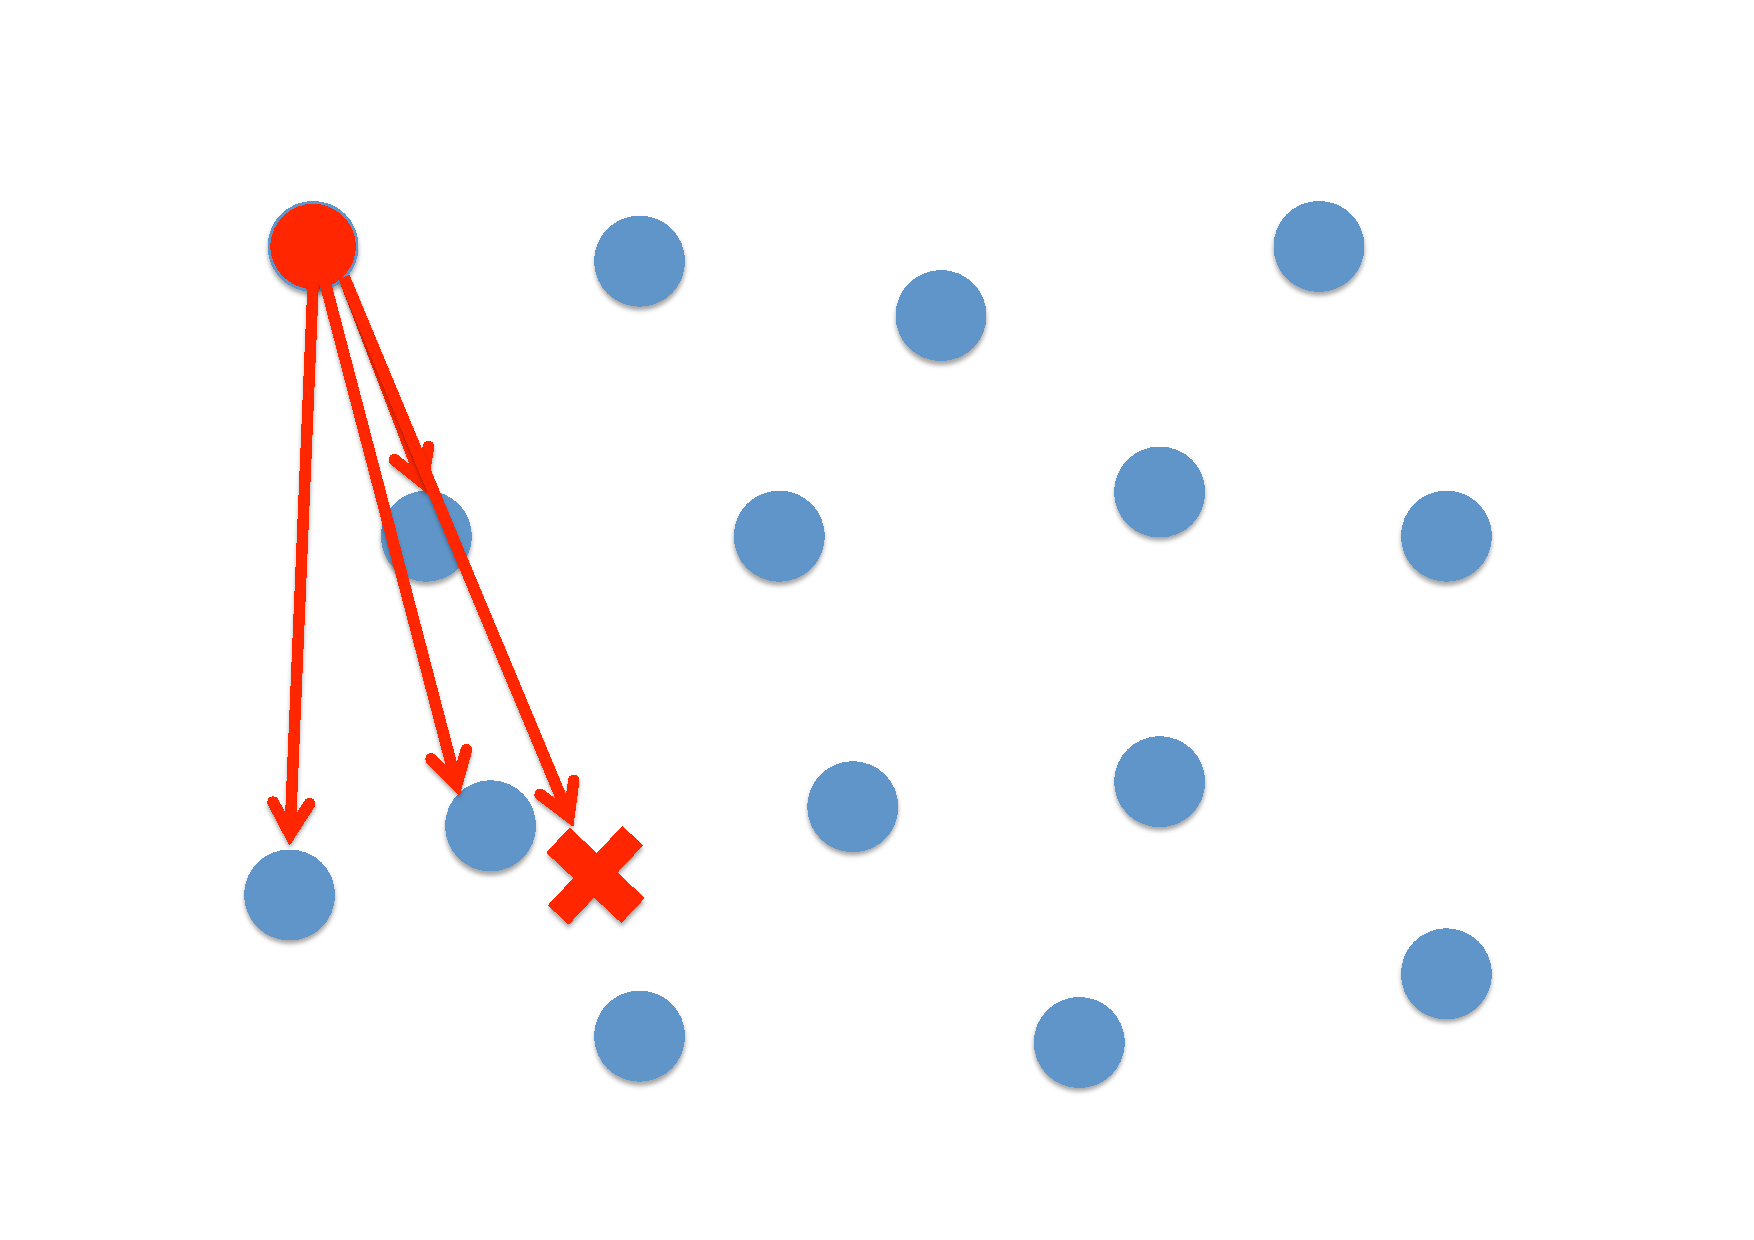
\includegraphics[width=1\textwidth]{pics/fault2}
  \end{center}
\end{figure}

}

\frame{
\frametitle{The Academic View: Data Dissemination}
\framesubtitle{Design Alternatives: One to All}

\begin{figure}[h]
  \begin{center}
  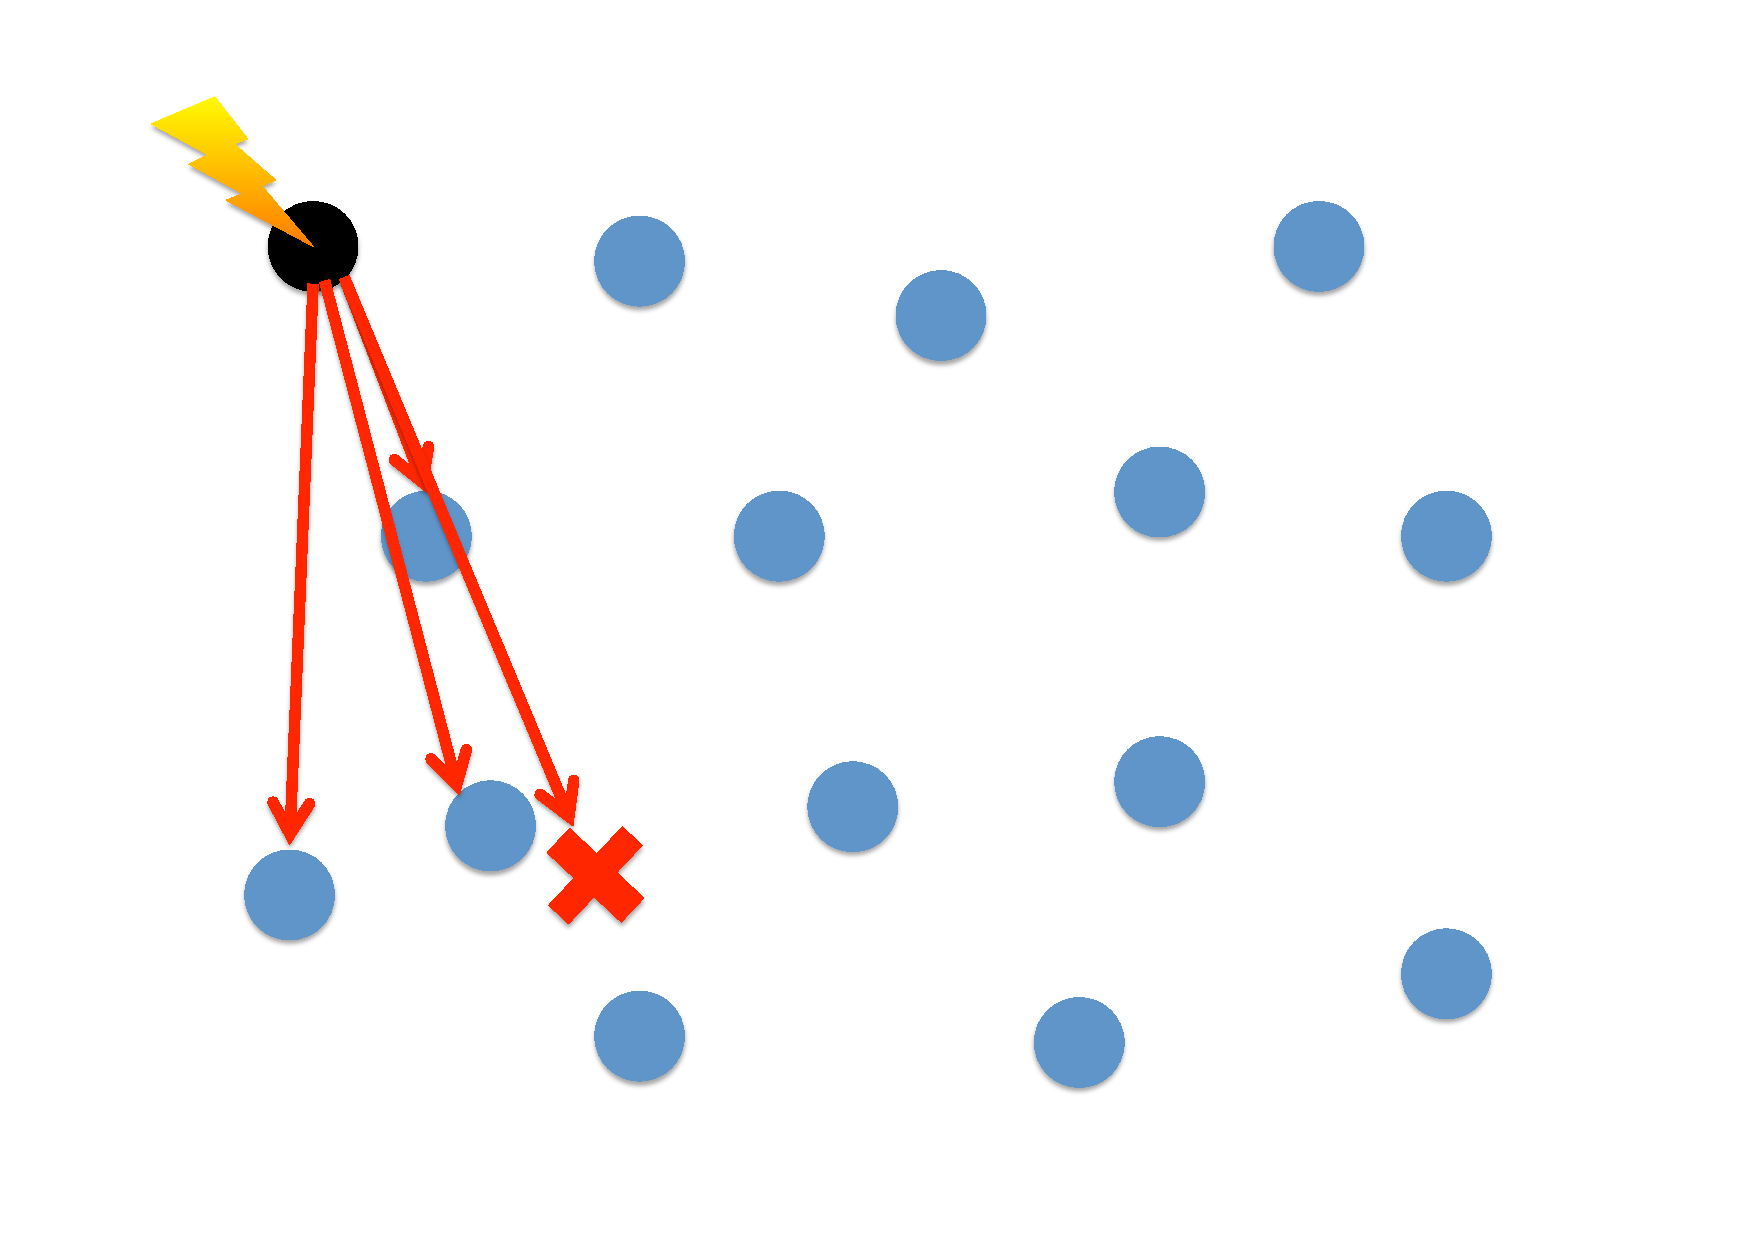
\includegraphics[width=1\textwidth]{pics/fault3}
  \end{center}
\end{figure}

}

\frame{
\frametitle{The Academic View: Data Dissemination}
\framesubtitle{Design Alternatives: One to All}

\begin{figure}[h]
  \begin{center}
  \includegraphics[width=1\textwidth]{pics/fault4}
  \end{center}
\end{figure}

}

\subsection{Design Alternatives: Spanning Tree}

\frame{
\frametitle{The Academic View: Data Dissemination}
\framesubtitle{Design Alternatives: Spanning Tree}

}

\subsection{Design Alternatives: Flood}

\frame{	
\frametitle{The Academic View: Data Dissemination}
\framesubtitle{Design Alternatives: Flood}

}

\subsection{Design Alternatives: Gossip}

\frame{
\frametitle{The Academic View: Data Dissemination}
\framesubtitle{Design Alternatives: Gossip}

}

\subsection{Design Alternatives: Embedded Tree}

\frame{
\frametitle{The Academic View: Data Dissemination}
\framesubtitle{Design Alternatives: Embedded Tree}

}

\section{Embedded Tree: Plumtree Protocol}

\frame{
\frametitle{Embedded Trees: Plumtree Protocol}
\framesubtitle{Building the Tree}

}


\frame{
\frametitle{Embedded Trees: Plumtree Protocol}
\framesubtitle{Recovering the Tree}

}


\frame{
\frametitle{Embedded Trees: Plumtree Protocol}
\framesubtitle{Sharing the Tree}

}

\frame{
\frametitle{Embedded Trees: Plumtree Protocol}
\framesubtitle{Experimental Evaluation}

}



\section{The Industry View: Cluster Metadata Management}

\frame
{
	\frametitle{Outline}
{
\small
	\tableofcontents[currentsection,hideallsubsections]
}
}

\frame{
\frametitle{The Industry View: Cluster Metadata Management}
\framesubtitle{}

}

%To Jordan: Add your sub sections / main slides here

\section{Cluster Metadata Management In Riak}

\frame
{
	\frametitle{Outline}
{
\small
	\tableofcontents[currentsection,hideallsubsections]
}
}

%To Jordan: Add your sub sections / main slides here

\frame{
\frametitle{Cluster Metadata Management In Riak}
\framesubtitle{}

}


\section{The Academic View: When One Tree is not Enough}

\frame
{
	\frametitle{Outline}
{
\small
	\tableofcontents[currentsection,hideallsubsections]
}
}

\subsection{Understanding The Problem}

\frame{
\frametitle{The Academic View: When One Tree is not Enough}
\framesubtitle{Understanding The Problem}

}

\subsection{Naive Solutions}

\frame{
\frametitle{The Academic View: When One Tree is not Enough}
\framesubtitle{Naive Solutions}

}


\subsection{Other Solutions}

\frame{
\frametitle{The Academic View: When One Tree is not Enough}
\framesubtitle{Other Solutions}

}

\subsection{Understanding The Goal}

\frame{
\frametitle{The Academic View: When One Tree is not Enough}
\framesubtitle{Understanding The Goal}

}


\section{The Thicket Protocol}

\frame
{
	\frametitle{Outline}
{
\small
	\tableofcontents[currentsection,hideallsubsections]
}
}

\subsection{Deploying the Trees}

\frame{
\frametitle{The Thicket Protocol}
\framesubtitle{Deploying the Trees}

}

\subsection{Recovering Trees}

\frame{
\frametitle{The Thicket Protocol}
\framesubtitle{Recovering Trees}

}

\subsection{Experimental Results}

\frame{
\frametitle{The Thicket Protocol}
\framesubtitle{Experimental Results}

}

\section{The Industry View: Improving Cluster Metadata Management}

%To Jordan: Add your sub sections / main slides here

\frame
{
	\frametitle{Outline}
{
\small
	\tableofcontents[currentsection,hideallsubsections]
}
}

\frame{
\frametitle{The Industry View: Improving Cluster Metadata Management}
\framesubtitle{}

}

\section{The Future of Cluster Metadata Management in Riak}

%To Jordan: Add your sub sections / main slides here

\frame
{
	\frametitle{Outline}
{
\small
	\tableofcontents[currentsection,hideallsubsections]
}
}

\frame{
\frametitle{The Future of Cluster Metadata Management in Riak}
\framesubtitle{}

}

\section{Summary}

\frame
{
	\frametitle{Outline}
{
\small
	\tableofcontents[currentsection,hideallsubsections]
}
}

\frame{
\frametitle{Summary}
\framesubtitle{}

}

\frame
{
	\frametitle{}
	\framesubtitle{}
	
	\begin{center}
		{\Huge
			Thanks.
		}
	\end{center}	
}

\end{document}
